\documentclass[tikz,border=2pt]{standalone}
\usetikzlibrary{arrows.meta}
\begin{document}
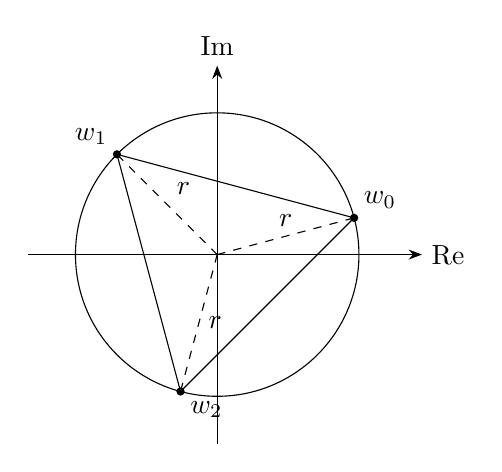
\begin{tikzpicture}[>=Stealth]
    \def\R{1.8}
    \draw[->] (-2.4,0) -- (2.6,0) node[right] {$\mathrm{Re}$};
    \draw[->] (0,-2.4) -- (0,2.4) node[above] {$\mathrm{Im}$};
    \draw (0,0) circle (\R);
    \coordinate (W0) at (15:\R);
    \coordinate (W1) at (135:\R);
    \coordinate (W2) at (255:\R);
    \draw (W0) -- (W1) -- (W2) -- cycle;
    \draw[dashed] (0,0) -- (W0) node[midway,above] {$r$};
    \draw[dashed] (0,0) -- (W1) node[midway,above right] {$r$};
    \draw[dashed] (0,0) -- (W2) node[midway,right] {$r$};
    \foreach \p/\a/\n in {W0/15/0,W1/135/1,W2/255/2}{
        \fill (\p) circle (1.5pt);
    }
    \node[above right] at (W0) {$w_0$};
    \node[above left]  at (W1) {$w_1$};
    \node[below right] at (W2) {$w_2$};
\end{tikzpicture}
\end{document}
